%% abtex2-modelo-trabalho-academico.tex, v-1.9.7 laurocesar
%% Copyright 2012-2018 by abnTeX2 group at http://www.abntex.net.br/ 
%%
%% This work may be distributed and/or modified under the
%% conditions of the LaTeX Project Public License, either version 1.3
%% of this license or (at your option) any later version.
%% The latest version of this license is in
%%   http://www.latex-project.org/lppl.txt
%% and version 1.3 or later is part of all distributions of LaTeX
%% version 2005/12/01 or later.
%%
%% This work has the LPPL maintenance status `maintained'.
%% 
%% The Current Maintainer of this work is the abnTeX2 team, led
%% by Lauro César Araujo. Further information are available on 
%% http://www.abntex.net.br/
%%
%% This work consists of the files abntex2-modelo-trabalho-academico.tex,
%% abntex2-modelo-include-comandos and abntex2-modelo-references.bib
%%

% ------------------------------------------------------------------------
% ------------------------------------------------------------------------
% abnTeX2: Modelo de Trabalho Academico (tese de doutorado, dissertacao de
% mestrado e trabalhos monograficos em geral) em conformidade com 
% ABNT NBR 14724:2011: Informacao e documentacao - Trabalhos academicos -
% Apresentacao
% ------------------------------------------------------------------------
% ------------------------------------------------------------------------

\documentclass[
	% -- opções da classe memoir --
	12pt,				 % tamanho da fonte
	oneside,			 % para impressão em recto.
	a4paper,			 % tamanho do papel.
	% -- opções da classe abntex2 --
	chapter=TITLE,		 % títulos de capítulos convertidos em letras maiúsculas
	section=TITLE,		 % títulos de seções convertidos em letras maiúsculas
	sumario=tradicional, % estilo do sumário (tradicional = indentado)
	% -- opções do pacote babel --
	english,			 % idioma adicional para hifenização
	brazil				 % o último idioma é o principal do documento
	]{abntex2}

% ---
% Pacotes básicos 
% ---
\usepackage{helvet}			    % Usa a fonte Helvet			
\usepackage[T1]{fontenc}		% Selecao de codigos de fonte.
\usepackage[utf8]{inputenc}		% Codificacao do documento (conversão automática dos acentos)
\usepackage{indentfirst}		% Indenta o primeiro parágrafo de cada seção.
\usepackage{color}				% Controle das cores
\usepackage{graphicx}			% Inclusão de gráficos
\usepackage{microtype} 			% Para melhorias de justificação
\usepackage{lib/unifacens}      % Adaptações as normas da UniFacens
\usepackage{pdfpages}           % Para incluir pdf no documento
\usepackage{ragged2e}           % Para alinhamento de texto
\usepackage{titlesec}           % Para estilo dos capítulos/subcapítulos
\usepackage[bottom]{footmisc}   % arruma posição da nota de rodapé
% ---
		
% ---
% Pacotes adicionais, usados apenas no âmbito do Modelo Canônico do abnteX2
% ---
\usepackage{lipsum}				% para geração de dummy text
% ---

% ---
% Pacotes de citações
% ---
\usepackage[alf]{abntex2cite}	% Citações padrão ABNT
\usepackage{lib/url6023} % remove < > nas urls

% --- 
% CONFIGURAÇÕES DE ESTILO E TAMANHO DA FONTE
% --- 

% Define a fonte padrão como serif (Arial)
\renewcommand{\familydefault}{\sfdefault}

% Define o tamanho da fonte dos capitulos para 14pt.
\renewcommand*{\chapnumfont}{\normalfont\large\bfseries\sffamily}
\renewcommand*{\chaptitlefont}{\normalfont\large\bfseries\sffamily}

% Define o tamanho da fonte das seções e sub-seções para 12pt,
% sendo as seções em negrito.
\setsecheadstyle{\normalsize}
\setsubsecheadstyle{\normalsize}
% ---

\makeatletter
\titleformat{\section}
  {\MakeUppercase}{\thesection}{1em}{}
\makeatother

\graphicspath{{./images/}}

% ---
% Informações sobre o trabalho
% ---
\coordenadoria{Coordenadoria de Engenharia da Computação}
\titulo{Titulo do trabalho}
\subtitulo{Subtitulo se houver}
\integranteum{Nome do aluno 1}
\integrantedois{Nome do aluno 2}
\local{Sorocaba/SP}
\data{2021}

% ---
% Informações sobre orientador
% ---
\orientador{Nome do orientador}

% ---
% Informações sobre coorientador
% ---
\coorientador{}

% O preambulo deve conter o tipo do trabalho, o objetivo, 
% o nome da instituição e a área de concentração 
\preambulo{Trabalho de conclusão de curso apresentado ao Centro Universitário Facens como exigência parcial para obtenção do diploma de graduação em Engenharia da Computação.\\ Orientador: Prof. ---------------------------}
% ---


% ---
% Configurações de aparência do PDF final

% alterando o aspecto da cor azul
\definecolor{blue}{RGB}{41,5,195}

% informações do PDF
\makeatletter
\hypersetup{
     	%pagebackref=true,
		pdftitle={\@title}, 
		pdfauthor={\@author},
    	pdfsubject={\imprimirpreambulo},
	    pdfcreator={LaTeX with abnTeX2},
		pdfkeywords={abnt}{latex}{abntex}{abntex2}{trabalho acadêmico}, 
		colorlinks=true,       		% false: boxed links; true: colored links
    	linkcolor=black,          	% color of internal links
    	citecolor=blue,        		% color of links to bibliography
    	filecolor=magenta,      		% color of file links
		urlcolor=blue,
		bookmarksdepth=4
}
\makeatother
% --- 

% ---
% Posiciona figuras e tabelas no topo da página quando adicionadas sozinhas
% em um página em branco. Ver https://github.com/abntex/abntex2/issues/170
\makeatletter
\setlength{\@fptop}{5pt} % Set distance from top of page to first float
\makeatother
% ---

% ---
% Possibilita criação de Quadros e Lista de quadros.
% Ver https://github.com/abntex/abntex2/issues/176
%
\newcommand{\quadroname}{Quadro}
\newcommand{\listofquadrosname}{Lista de quadros}

\newfloat[chapter]{quadro}{loq}{\quadroname}
\newlistof{listofquadros}{loq}{\listofquadrosname}
\newlistentry{quadro}{loq}{0}

% configurações para atender às regras da ABNT
\setfloatadjustment{quadro}{\centering}
\counterwithout{quadro}{chapter}
\renewcommand{\cftquadroname}{\quadroname\space} 
\renewcommand*{\cftquadroaftersnum}{\hfill--\hfill}

\setfloatlocations{quadro}{hbtp} % Ver https://github.com/abntex/abntex2/issues/176
% ---

% ---
% Adaptações para atender o sumário da biblioteca FACENS
%

% Define os capítulos como caixa alta
\makeatletter
\settocpreprocessor{chapter}{%
    \let\tempf@rtoc\f@rtoc% 
    \def\f@rtoc{%
      \texorpdfstring{\MakeTextUppercase{%
        \tempf@rtoc}%
      }{\tempf@rtoc}%
    }% 
}
\makeatother

% define seções como caixa alta
\makeatletter
\let\oldcontentsline\contentsline
\def\contentsline#1#2{%
  \expandafter\ifx\csname l@#1\endcsname\l@section
    \expandafter\@firstoftwo
  \else
    \expandafter\@secondoftwo
  \fi
  {%
    \oldcontentsline{#1}{\MakeTextUppercase{#2}}%
  }{%
    \oldcontentsline{#1}{#2}%
  }%
}
\makeatother

% remove identação sumário
\cftsetindents{chapter}{0cm}{0.5cm}
\cftsetindents{section}{0cm}{0.8cm}
\cftsetindents{subsection}{0cm}{1.1cm}

% altera fonte do capitulo de referencias para caixa alta no sumário
\renewcommand{\bibsection}{%
    \chapter*{\bibname}
    \bibmark
    \ifnobibintoc\else
    \phantomsection
    \addcontentsline{toc}{chapter}{\uppercase{\bibname}}
    \fi
    \prebibhook
}
%---

\usepackage{float}

% --- 
% Espaçamentos entre linhas e parágrafos 
% --- 

% O tamanho do parágrafo é dado por:
\setlength{\parindent}{1.3cm}

% Controle do espaçamento entre um parágrafo e outro:
\setlength{\parskip}{0.2cm}  % tente também \onelineskip

% Controle do espaçamento após um capitulo, seção e sub-seção
\setlength{\afterchapskip}{\baselineskip}
\setlength{\aftersecskip}{\baselineskip}
\setlength{\aftersubsecskip}{\baselineskip}

% ---
% compila o indice
% ---
\makeindex
% ---

% remove header pagina impar
\makepagestyle{cabecalhopaginaimpar}
  %%cabeçalhos
  \makeoddhead{cabecalhopaginaimpar} %% pagina ímpar ou com oneside
    {}{}{\small\thepage}

% ----
% Início do documento
% ----
\begin{document}

% Seleciona o idioma do documento (conforme pacotes do babel)
%\selectlanguage{english}
\selectlanguage{brazil}

% Retira espaço extra obsoleto entre as frases.
\frenchspacing 

% ----------------------------------------------------------
% ELEMENTOS PRÉ-TEXTUAIS
% ----------------------------------------------------------
\imprimircapa
\imprimirfolhaderosto*

\begin{fichacatalografica}
	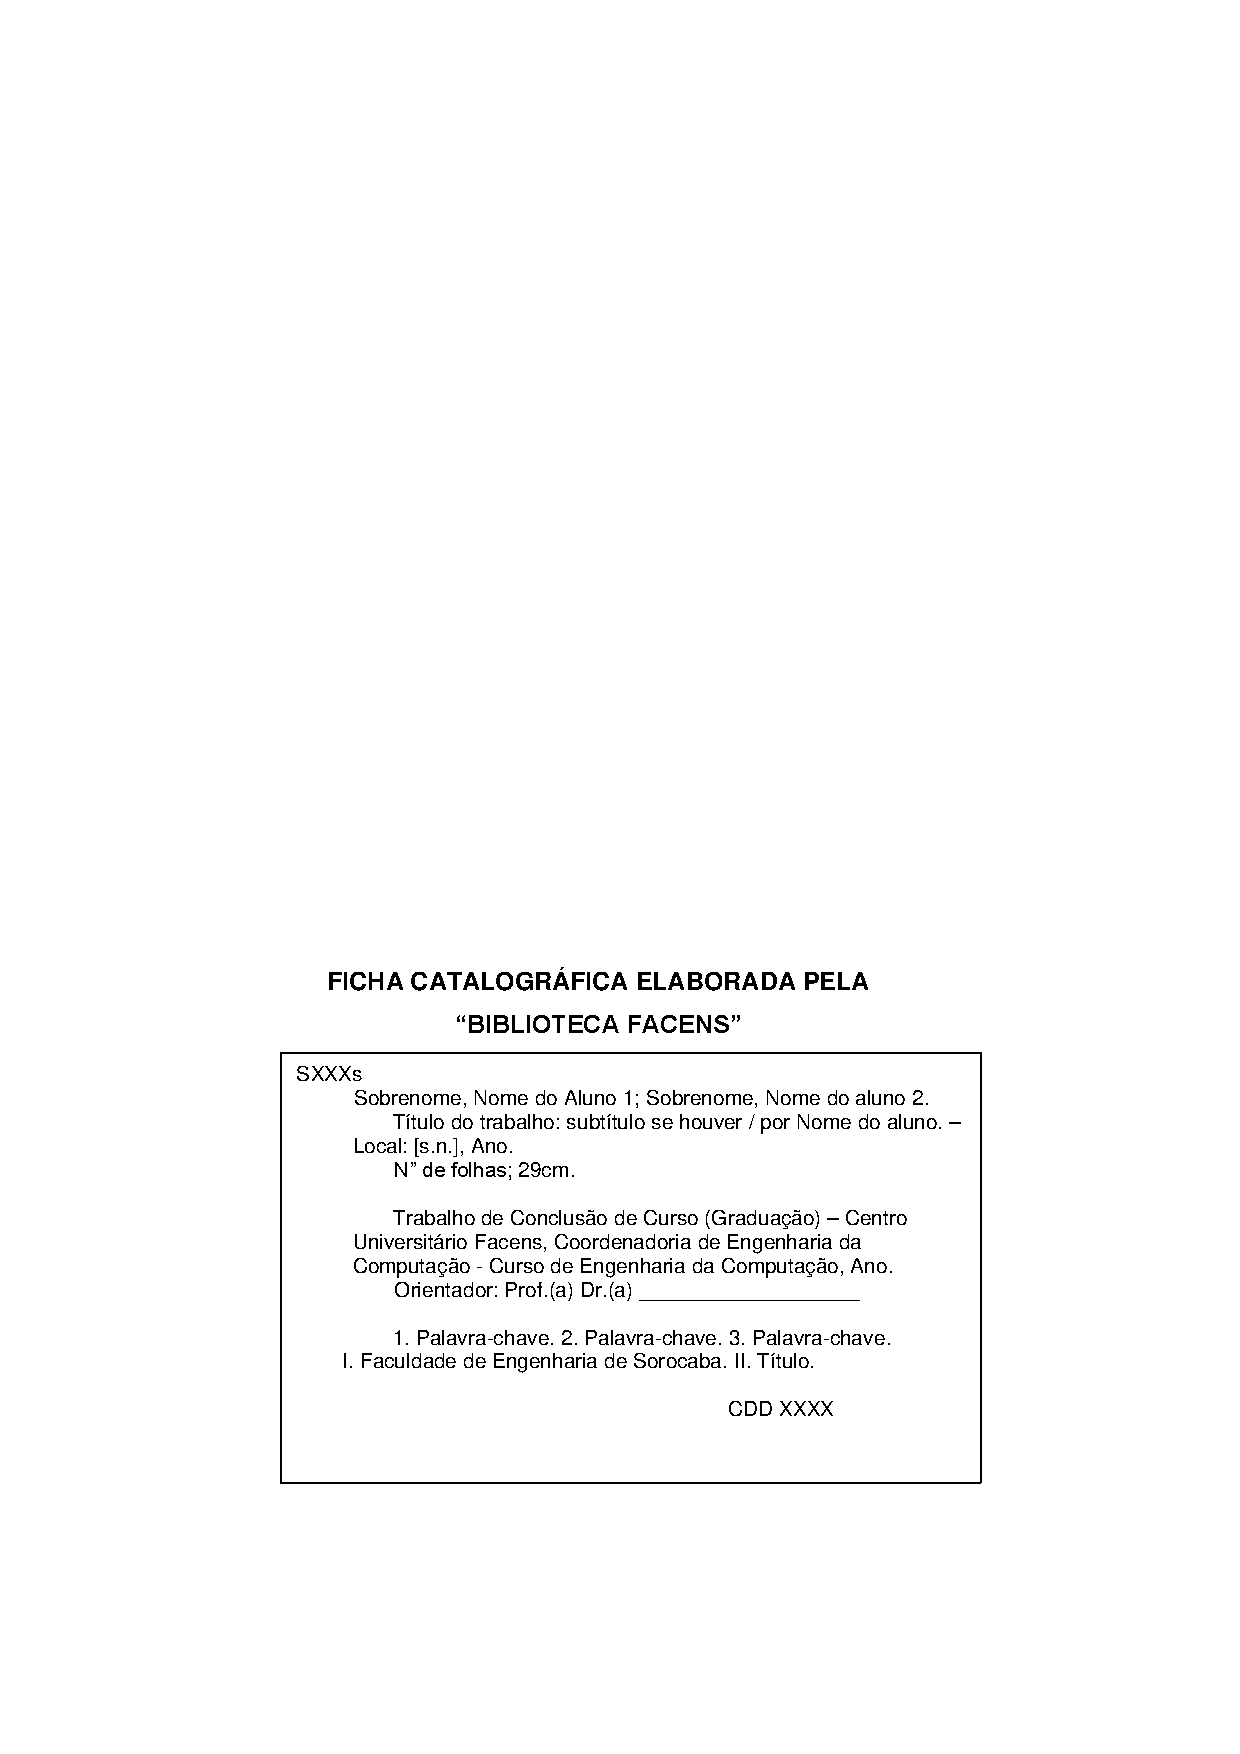
\includepdf[page=1]{partes/pre_textuais/ficha_catalografica.pdf}
\end{fichacatalografica}
\begin{folhadeaprovacao}
	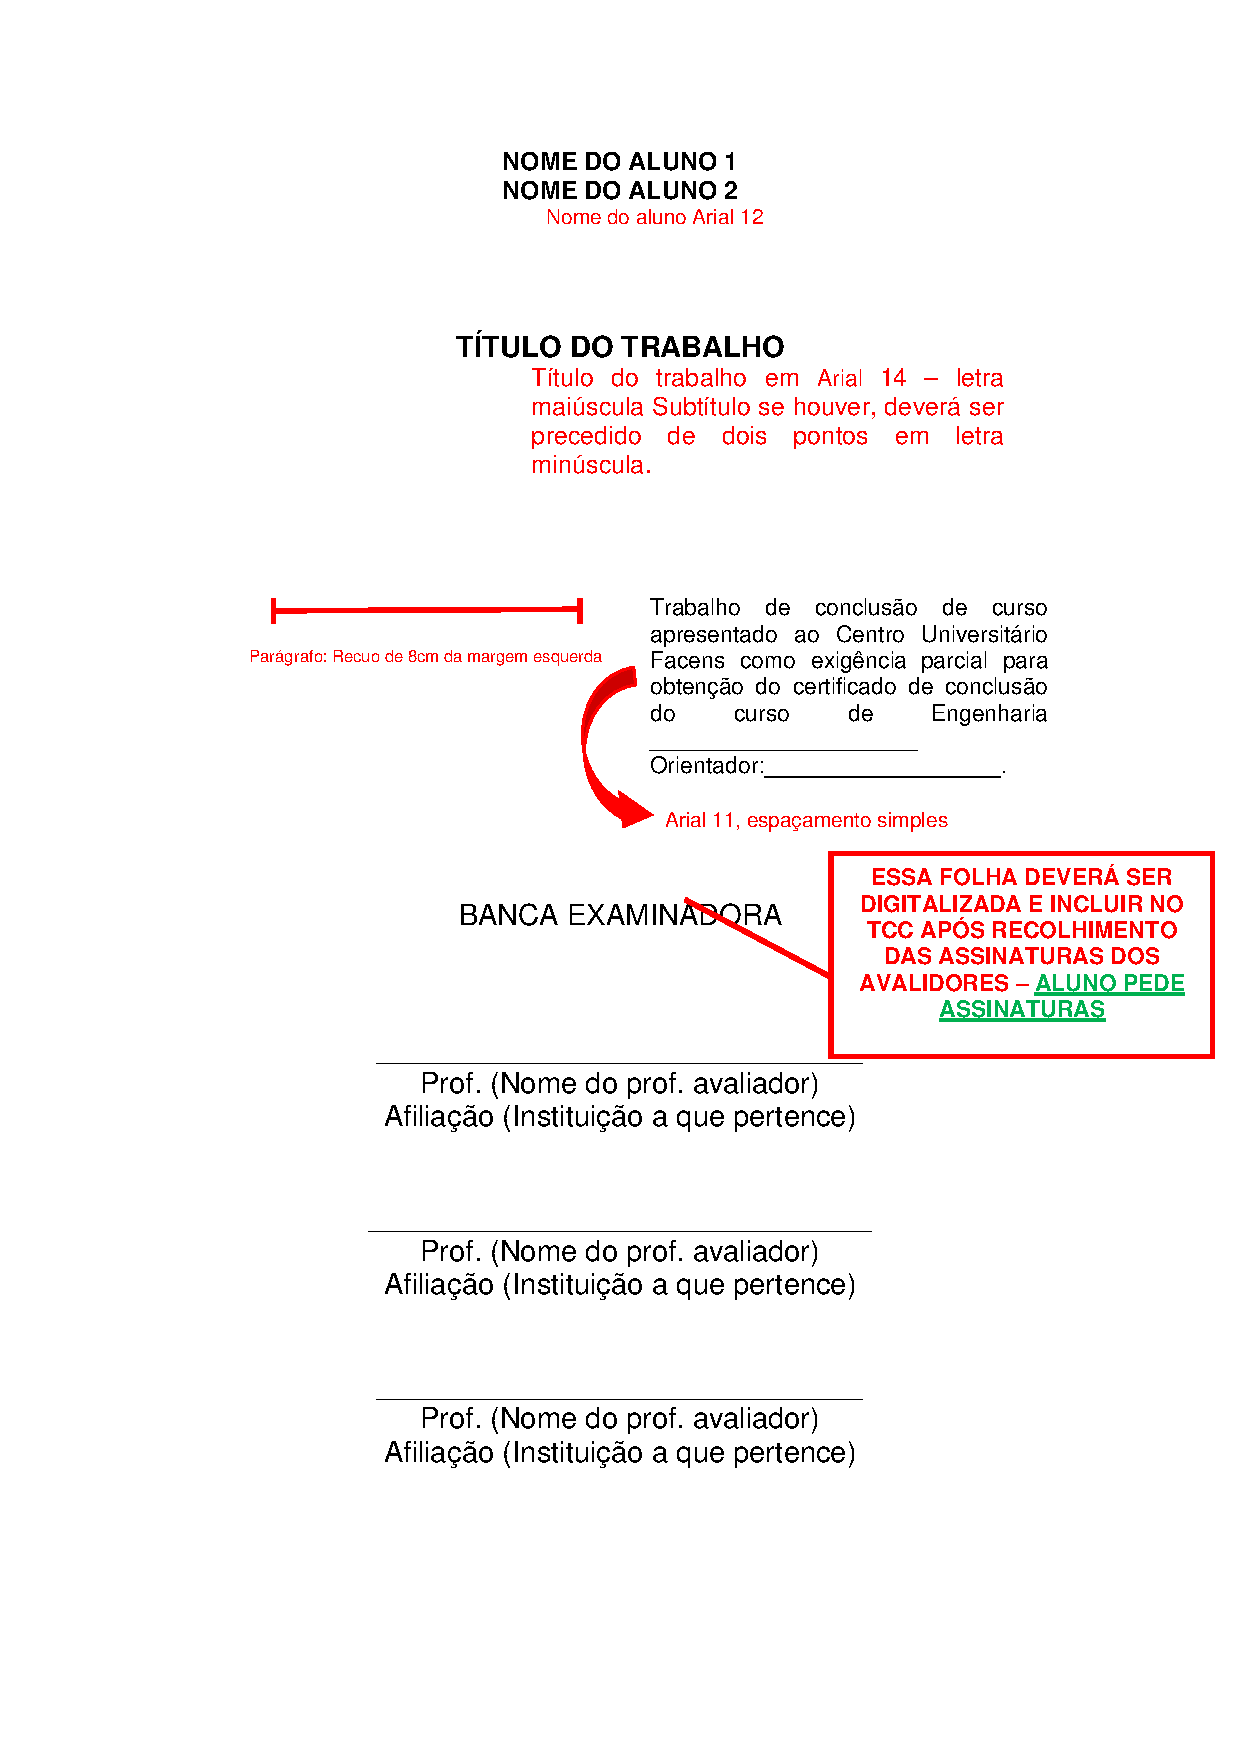
\includepdf[page=1]{partes/pre_textuais/folha_aprovacao.pdf}
\end{folhadeaprovacao}
\begin{agradecimentos}
    Os agradecimentos principais são direcionados à Gerald Weber, Miguel Frasson,
    Leslie H. Watter, Bruno Parente Lima, Flávio de Vasconcellos Corrêa, Otavio Real
    Salvador, Renato Machnievscz e todos aqueles que
    contribuíram para que a produção de trabalhos acadêmicos conforme
    as normas ABNT com \LaTeX\ fosse possível.

    Agradecimentos especiais são direcionados ao Centro de Pesquisa em Arquitetura
    da Informação da Universidade de
    Brasília (CPAI), ao grupo de usuários
    \emph{latex-br} e aos
    novos voluntários do grupo
    \emph{\abnTeX} e que contribuíram e que ainda
    contribuirão para a evolução do \abnTeX.
\end{agradecimentos}
\begin{epigrafe}
    \vspace*{\fill}
    
    \begin{flushright}
        \begin{minipage}{8cm}
            \begin{SingleSpace}
                ``Não vos amoldeis às estruturas deste mundo,
                mas transformai-vos pela renovação da mente,
                a fim de distinguir qual é a vontade de Deus:
                o que é bom, o que Lhe é agradável, o que é perfeito.``\\
                (Bíblia Sagrada, Romanos 12, 2)
            \end{SingleSpace}
        \end{minipage}
    \end{flushright}
\end{epigrafe}
% resumo em português
\setlength{\absparsep}{18pt} % ajusta o espaçamento dos parágrafos do resumo
\begin{resumo}
    Segundo a \citeonline[3.1-3.2]{NBR6028:2003}, o resumo deve ressaltar o
    objetivo, o método, os resultados e as conclusões do documento. A ordem e a extensão
    destes itens dependem do tipo de resumo (informativo ou indicativo) e do
    tratamento que cada item recebe no documento original. O resumo deve ser
    precedido da referência do documento, com exceção do resumo inserido no
    próprio documento. (\ldots) As palavras-chave devem figurar logo abaixo do
    resumo, antecedidas da expressão Palavras-chave:, separadas entre si por
    ponto e finalizadas também por ponto.

    \textbf{Palavras-chave}: latex. abntex. editoração de texto.
\end{resumo}

% resumo em inglês
\begin{resumo}[Abstract]
    \begin{otherlanguage*}{english}
        This is the english abstract.

        \vspace{\onelineskip}

        \noindent 
        \textbf{Keywords}: latex. abntex. text editoration.
    \end{otherlanguage*}
\end{resumo}
\pdfbookmark[0]{\listfigurename}{lof}
\listoffigures*
\cleardoublepage
\pdfbookmark[0]{\listofquadrosname}{loq}
\listofquadros*
\cleardoublepage
\pdfbookmark[0]{\listtablename}{lot}
\listoftables*
\cleardoublepage
\begin{siglas}
    \item[ABNT] Associação Brasileira de Normas Técnicas
    \item[abnTeX] ABsurdas Normas para TeX
\end{siglas}
\pdfbookmark[0]{\contentsname}{toc}
\tableofcontents*
\cleardoublepage

% ----------------------------------------------------------
% ELEMENTOS TEXTUAIS
% ----------------------------------------------------------
\textual
\pagestyle{cabecalhopaginaimpar}

\chapter{Introdução}
% ----------------------------------------------------------

Este documento e seu código-fonte são exemplos de referência de uso da classe
\textsf{abntex2} e do pacote \textsf{abntex2cite}. O documento 
exemplifica a elaboração de trabalho acadêmico (tese, dissertação e outros do
gênero) produzido conforme a ABNT NBR 14724:2011 \emph{Informação e documentação
- Trabalhos acadêmicos - Apresentação}.

A expressão ``Modelo Canônico'' é utilizada para indicar que \abnTeX\ não é
modelo específico de nenhuma universidade ou instituição, mas que implementa tão
somente os requisitos das normas da ABNT. Uma lista completa das normas
observadas pelo \abnTeX\ é apresentada em \citeonline{abntex2classe}.

Sinta-se convidado a participar do projeto \abnTeX! Acesse o site do projeto em
\url{http://www.abntex.net.br/}. Também fique livre para conhecer,
estudar, alterar e redistribuir o trabalho do \abnTeX, desde que os arquivos
modificados tenham seus nomes alterados e que os créditos sejam dados aos
autores originais, nos termos da ``The \LaTeX\ Project Public
License''\footnote{\url{http://www.latex-project.org/lppl.txt}}.

Encorajamos que sejam realizadas customizações específicas deste exemplo para
universidades e outras instituições --- como capas, folha de aprovação, etc.
Porém, recomendamos que ao invés de se alterar diretamente os arquivos do
\abnTeX, distribua-se arquivos com as respectivas customizações.
Isso permite que futuras versões do \abnTeX~não se tornem automaticamente
incompatíveis com as customizações promovidas. Consulte
\citeonline{abntex2-wiki-como-customizar} para mais informações.

Este documento deve ser utilizado como complemento dos manuais do \abnTeX\ 
\cite{abntex2classe,abntex2cite,abntex2cite-alf} e da classe \textsf{memoir}
\cite{memoir}. 

Esperamos, sinceramente, que o \abnTeX\ aprimore a qualidade do trabalho que
você produzirá, de modo que o principal esforço seja concentrado no principal:
na contribuição científica.

Equipe \abnTeX 

Lauro César Araujo
\include{abntex2-modelo-include-comandos}

\chapter{Referencial teórico}\label{cap_trabalho_academico}

\section{Aliquam vestibulum fringilla lorem}

\lipsum[1]

\subsection{Pellentesque sit amet pede ac sem eleifend consectetuer}
\lipsum[2-3]
\chapter{Desenvolvimento}

\section{Quadros}

Este modelo vem com o ambiente \texttt{quadro} e impressão de Lista de quadros 
configurados por padrão. Verifique um exemplo de utilização:

\begin{quadro}[htb]
    \caption{\label{quadro_exemplo}Exemplo de quadro}
    \begin{tabular}{|c|c|c|c|}
        \hline
        \textbf{Pessoa} & \textbf{Idade} & \textbf{Peso} & \textbf{Altura} \\ \hline
        Marcos & 26    & 68   & 178    \\ \hline
        Ivone  & 22    & 57   & 162    \\ \hline
        ...    & ...   & ...  & ...    \\ \hline
        Sueli  & 40    & 65   & 153    \\ \hline
    \end{tabular}
    \fonte{Autor.}
\end{quadro}

Este parágrafo apresenta como referenciar o quadro no texto, requisito
obrigatório da ABNT. 
Primeira opção, utilizando \texttt{autoref}: Ver o \autoref{quadro_exemplo}. 
Segunda opção, utilizando  \texttt{ref}: Ver o Quadro \ref{quadro_exemplo}.
% ---
% primeiro capitulo de Resultados
% ---
\chapter{Resultados}
% ---

% ---
\section{Vestibulum ante ipsum primis in faucibus orci luctus et ultrices
posuere cubilia Curae}
% ---

\lipsum[21-22]
\chapter{Considerações finais}
% ---

\lipsum[31-33]

% ----------------------------------------------------------
% ELEMENTOS PÓS-TEXTUAIS
% ----------------------------------------------------------
\titleformat{\chapter}
    {\large\bfseries\MakeUppercase}
    {}
    {}
    {}
\titlespacing*{\chapter}{0pt}{-22pt}{*3}
\bibliography{abntex2-modelo-references}

\begin{apendicesenv}

    \newpage
    \phantomsection
    
    \addcontentsline{toc}{chapter}{APÊNDICES}
    \addtocontents{toc}{\protect\setcounter{tocdepth}{-1}}
    
    \chapter{Quisque libero justo}
    \lipsum[50]

    \chapter{Nullam elementum urna vel imperdiet sodales elit ipsum pharetra ligula
    ac pretium ante justo a nulla curabitur tristique arcu eu metus}
    \lipsum[55-57]

    \addtocontents{toc}{\protect\setcounter{tocdepth}{0}}

\end{apendicesenv}
\begin{anexosenv}

    \newpage
    \phantomsection

    \addcontentsline{toc}{chapter}{ANEXOS}
    \addtocontents{toc}{\protect\setcounter{tocdepth}{-1}}
    
    % coloca o primeiro anexo na mesma pagina do titulo do capitulo
    \chapter{Morbi ultrices rutrum lorem}
    \lipsum[30]

    \chapter{Cras non urna sed feugiat cum sociis natoque penatibus et magnis dis
    parturient montes nascetur ridiculus mus}
    \lipsum[31]

    \chapter{Fusce facilisis lacinia dui}
    \lipsum[32]

    \addtocontents{toc}{\protect\setcounter{tocdepth}{0}}

\end{anexosenv}

%---------------------------------------------------------------------
% INDICE REMISSIVO
%---------------------------------------------------------------------
\printindex
%---------------------------------------------------------------------

\end{document}
